\documentclass[12pt, a4paper, twoside, romanian]{teza-upb}
\setcounter{secnumdepth}{3}
\setcounter{tocdepth}{3}
\usepackage{babel}
\usepackage{graphicx}
\usepackage{amsthm}
\usepackage{pbox}
\usepackage{amsfonts}
\usepackage{amsmath}
\usepackage{url}
\usepackage{minted}
\usepackage{fca}
\usepackage{algorithm}
\usepackage[noend]{algpseudocode}
\graphicspath{ {images/} }
\usepackage[
  bookmarksnumbered,
  bookmarks,
  bookmarksopen=true,
  pdftitle={Licența Chereji Mihai},
  linktocpage
  ]{hyperref}

%\singlespacing
\newtheorem{defn}{Definiție}
\newtheorem{example}{Exemplu}
\newtheorem{theorem}{Teoremă}
\linespread{1.15}

\floatname{algorithm}{Algoritm}
\renewcommand{\algorithmicrequire}{\textbf{Date de intrare:}}
\renewcommand{\algorithmicensure}{\textbf{Date de ieșire:}}
\algrenewcommand{\algorithmicfunction}{\textbf{funcție}}
\algrenewcommand{\algorithmicreturn}{\textbf{întoarce}}
\algrenewcommand{\algorithmicwhile}{\textbf{cât timp}}
\algrenewcommand{\algorithmicend}{\textbf{sfârșit}}
\algrenewcommand{\algorithmicdo}{\textbf{execută}}
\algrenewcommand{\algorithmicfor}{\textbf{pentru}}
\algrenewcommand{\algorithmicif}{\textbf{dacă}}

\begin{document}

\author{Mihai Chereji}

\title{Romagna: o abordare modernă asupra uneltelor de analiză conceptuală a datelor}


\facultatea{Facultatea de Electronică, Telecomunicații și Tehnologia Informației}
\tiplucrare{licență}
\domeniu{Calculatoare și tehnologia informației}
\catedra{Telecomunicații}
\program{Ingineria informației}
\titlulobtinut{Inginer}
\director{Christian Săcarea} 

\submissionmonth{Iulie} 
\submissionyear{2014} 

\beforepreface
\listoffigures
\listoftables
\abbreviations{ 
  DOM = Document Object Model \\
  HTML = HyperText Markup Language (limbaj de marcaj hiper-textual)\\
  FCA = Formal Concept Analysis (Analiza Conceptuală Formală)\\
  LLVM = Low Level Virtual Machine (Mașină virtuală la nivel scăzut)\\
  MVC = Model View Controller (Model Vedere Controlor) \\
  SVG = Scalable Vector Graphics (Grafice Scalabile Vectoriale)\\
  SQL = Structured Query Language (Limbaj de Interogare Structurată)\\
  XML = eXtendable Markup Language (Limbaj extensibil de marcaj)\\
}
\afterpreface 

\chapter*{Introducere}

  Big-data a devenit un domeniu foarte căutat în zilele noastre, devenit un cuvânt repetat de toată lumea, de la programatori la oameni de marketing. 
  Acest lucru se-ntâmplă deoarece lumea se \textit{îneacă} în date, adunate din diferite surse. Site-urile înregistrează fiecare mișcare a utilizatorilor, pedometre care încarcă pe Internet numărul de pași făcut de utilizator în fiecare oră, aparatele de analiză medicală întorc tot mai multe date.

  Interpretarea lor devine din ce în ce mai grea, și tendința este de a se folosi metode de \textit{machine learning}, ceea ce presupune învățarea automată a calculatoarelor prin prelucrarea repetată a unei cantități imense de date. . 
  
  \textbf{Analiza conceptuală formală} oferă o alternativă, în care adunarea datelor este automată dar prelucrarea și interpretarea datelor este realizată de om, bazându-se pe câteva principii matematice bine definite și (relativ) ușor de înțeles. 


Pe scurt, analiza conceptuală formală dezvoltă o metodă care este folosită în principal pentru a analiza date. Altfel spus, prin această metodă se pot deriva relații implicite între obiecte care sunt descrise prin legături intre seturi de atribute. Conceptele se numesc așa deoarece datele sunt structurate în unități care sa reprezinta concepte ale gândirii umane, sau abstracții formale ale acestora, pe care un om va putea sa le interpreteze cu ușurința.

Analiza conceptuală formală mai poate fi definită și ca o metodă de clasificare conceptuală (clustering conceptual).

  Acest câmp a început în anii 80 la Universitatea din Darmstadt, ca o evoluție a teoriei clasice a laticelor. Între timp, s-a dezvoltat într-un câmp care adună tot mai mulți cercetători și își dovedește utilitatea practică dincolo de câmpul din care s-a tras și dincolo de matematica abstractă.

  Ce e mai spectaculos e că totul se bazează pe câteva idei simple, elegante, generale, frumoase am putea spune, încât duc aproape de \textit{filozofia platonică} (un concept este alăturarea unei mulțimi de obiecte descrise de unele proprietăți și mulțimea acelor proprietăți).

  Unele din cele mai utilizate rezultate ale acestei metode de analiză sunt laticele de concept, diagrame care reprezintă ierarhiile conceptelor descrise mai sus. 
  
  \begin{figure}[h!]
    \centering
    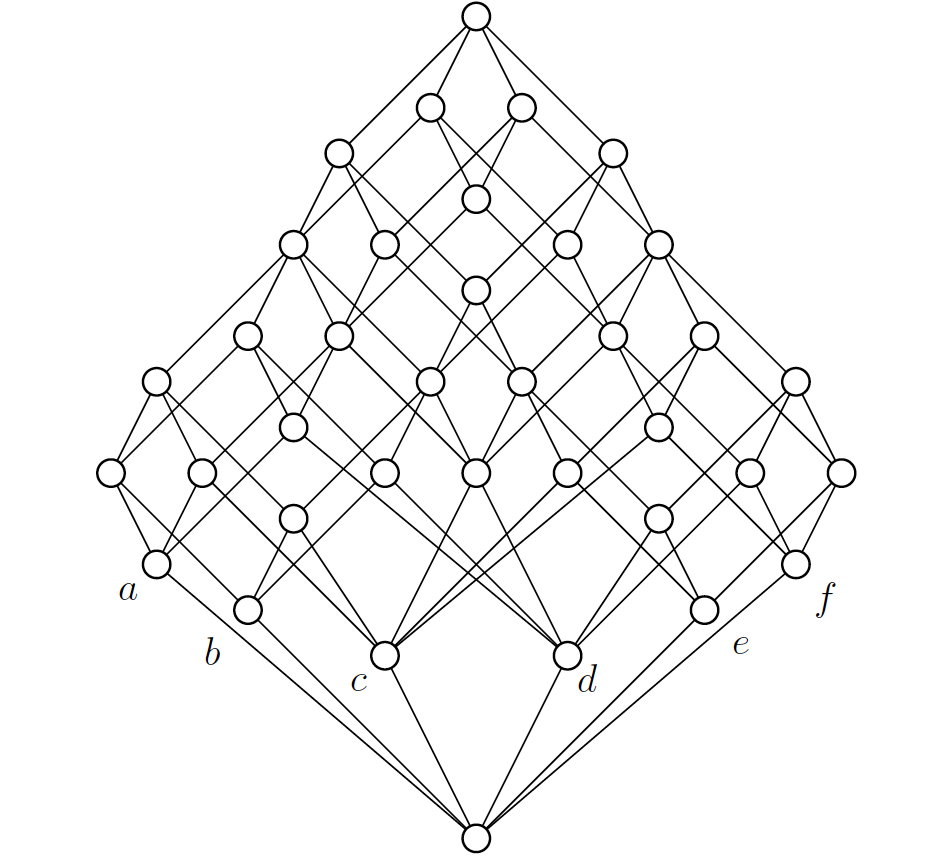
\includegraphics[width=0.6\textwidth, natwidth=944,natheight=864]{complete_lattice.png}
  \end{figure}
  Se observă că dincolo de utilitatea practică (descrisă în capitolele ce urmează), laticea este \textit{frumoasă}. Fără a încerca să-i descifreze înțelesul, oricine poate observa că este unul din acele produse ale științei care, neintenționat, poate fascina și studenții artelor.

  Cu toate acestea, domeniul analizei conceptuale formale duce lipsă de unelte frumoase (vom explica, în capitolele ce urmează ce înțelegem prin \textit{software frumos}), chiar dacă există tot mai multe programe care doresc să ajute cercetătorii în acest domeniu. Unele frustrează încă de la încercarea procesului de instalare, altele mistifică cercetătorul prin mesaje de eroare criptice, iar altele, poate, doar se mișcă prea încet, sau sunt prea greu de folosit.

  În cele ce urmează dorim să descriem pe scurt domeniul analizei conceptuale formale (în capitolul \ref{chapter:1}), starea soft-ului existent acum (în capitolul \ref{chapter:2}), tehnologiile folosite la dezvoltarea unei noi aplicații în capitolul \ref{chapter:3} și o viziune mai în detaliu asupra noii aplicații (capitolul \ref{chapter:4}), care dorește să rezolve unele din problemele întâlnite de oamenii interesați în acest domeniu, și poate, să atragă prin software bine gândit (și, sperăm, \textit{bine realizat}, căci un concept fără nici un obiect nu are cuprins - \textit{veți înțelege după ce veți parcurge primul capitol}) adepți noi.

\chapter{Analiza conceptuală formală}
\label{chapter:1}
  \section{Introducere}
    Analiza conceptuală formală este o metodă de sistematizare a datelor în \textbf{concepte}, definite la modul larg ca tupluri constituite din mulțimi de obiecte care împărtășesc anumite atribute și mulțimea acelor atribute. Este o reinterpretare a teoriei clasică a laticelor, dezvoltată în principal în anii '30, axată către partea practică. Conceptul a fost introdus în lucrarea seminală a lui Robert Wille din 1982 \cite{wille:1982}, iar termenul a fost introdus în 1984 de același autor. În ultimele decenii, domeniul a atras multe contribuții și și-a dovedit utilitatea în domenii cum ar fi analiza și vizualizarea datelor, managementul informației.
  \section{Concepte matematice de bază}
    Pentru a avea o mai bună înțelegere a conceptelor pe care se bazează aplicația, vom explica pe scurt definițiile de bază ale domeniului.
    \subsection{Mulțimi ordonate, latice, latice complete}
    Vom începe cu câteva concepte elementare de algebră a mulțimilor, deoarece acest domeniu se bazează în întregime pe ele. Următoarele definiții sunt preluate din \cite{Ganter:1997:FCA:550737}, înafara cazului unde este menționat altfel.
    \begin{defn}
      O mulțime $M$ este ordonată dacă se poate aplica asupra sa o relație binară $R$ care are următoarele proprietăți:
      \begin{description}
        \item [Reflexivitate] $xRx, \forall x \in M$
        \item [Antisimetrie] $xRy, x \neq y \Rightarrow yRx$ e fals, $\forall x, y \in M$
        \item [Tranzitivitate] $xRy, yRz \Rightarrow xRz, \forall x, y, z \in M$
      \end{description}
      Relația $R$ se numește o \textbf{relație de ordine}, sau \textbf{relație de ordine parțială}.
    \end{defn}

    Cel mai simplu exemplu, intuitiv exemplu este mulțimea numerelor reale $ \mathbb{R}$, alături de relația $\le$. Notăm o mulțime ordonată cu relația $\le$ cu $(M, \le)$. Un alt exemplu, relevant domeniului, este mulțimea tuturor submulțimilor sau \textit{mulțimea părților} a unei mulțimi (notată cu $\mathcal{P}(M)$ pentru mulțimea $M$), și relația de incluziune ($\subseteq$).

    \begin{defn}
      Un element $x$ al mulțimii $M$ este \textbf{acoperit} de $y$ dacă $x < y$ și nu există nici un $z$ astfel încât $x < z < y$. În mod invers, $x$ \textbf{acoperit} al lui $y$.
    \end{defn}

    Putem nota relația de acoperire astfel: $x \prec y, y \succ x$.

    \begin{defn}
      Două elemente ale unei mulțimi ordonate sunt \textbf{comparabile} (în raport cu $\le$) dacă $x \le y$ sau $y \le x$ (adică relația $\le$ se aplică asupra lor). Altfel sunt \textbf{incomparabile}. Un \textbf{lanț} este o submulțime în care oricare două elemente sunt comparabile. Un \textbf{antilanț} este o submulțime în care oricare două elemente sunt incomparabile.
    \end{defn}

    \begin{defn}
      \label{defn:hasse}
      \textbf{Diagramele Hasse} sunt o reprezentare grafică a unei mulțimi ordonate. Elementele mulțimii sunt desenate ca niște cercuri. Dacă $x, y \in M$ (mulțimea descrisă de diagramă) și $x \prec y$, se desenează o linie între cele două elemente, iar elementul acoperit este desenat sub cercul reprezentând elementul care îl acoperă.

      Astfel, putem citi o diagramă Hasse în felul următor: $x < y$ dacă și numai dacă putem urmări o linie continuă de la cercul care reprezintă $x$ la cercul care reprezintă $y$.
    \end{defn}

    \begin{example}
      Vom desena o diagramă Hasse reprezentând mulțimea de numere naturale\\ $\{ 1,2,3,4,5,6,10,12,15,20,30,60 \}$, ordonate după divizibilitate.
      \begin{figure}[h!]
        \centering
        \begin{minipage}{.65\textwidth}
          \unitlength 1.3mm
          \begin{diagram}{100}{52}
            \Node{1}{20}{0} \Node{2}{36}{12} \Node{3}{20}{12}
            \Node{4}{52}{24} \Node{5}{4}{12} \Node{6}{36}{24}
            \Node{7}{22}{24} %10
            \Node{8}{4}{24} % 15
            \Node{9}{40}{48}
            \Node{10}{52}{36} % 12
            \Node{11}{40}{36} %20
            \Node{12}{24}{36} %30
            \rightAttbox{9}{3}{-2}{60}
            \rightAttbox{1}{3}{-2}{1}
            \rightAttbox{2}{3}{-2}{2}
            \rightAttbox{3}{3}{-2}{3}
            \rightAttbox{4}{3}{-2}{4}
            \rightAttbox{5}{3}{-2}{5}
            \rightAttbox{6}{3}{-2}{6}
            \rightAttbox{7}{3}{-2}{10}
            \rightAttbox{8}{3}{-2}{15}
            \rightAttbox{10}{3}{-2}{12}
            \rightAttbox{11}{3}{-2}{20}
            \rightAttbox{12}{3}{-2}{30}
            \Edge{1}{2} \Edge{1}{3} \Edge{1}{5} \Edge{2}{4}
            \Edge{2}{6} \Edge{2}{7} \Edge{3}{6} \Edge{3}{8}
            \Edge{4}{10} \Edge{4}{11} \Edge{5}{7} \Edge{5}{8}
            \Edge{6}{10} \Edge{6}{12} \Edge{7}{11} \Edge{7}{12}
            \Edge{8}{12} \Edge{10}{9} \Edge{11}{9} \Edge{12}{9}
          \end{diagram}
        \end{minipage}
      \caption{Diagramă Hasse a unei mulțimi de numere naturale, ordonate după divizibiltate.}
      \end{figure}
    \end{example}

    \begin{defn}
      Fie $(M, \le)$ o mulțime ordonată, și $N$ o submulțime a sa. Înțelegem prin \textbf{minorantul} mulțimii $N$ un element $i$ astfel încât $\forall a \in N, i \le a$. În mod invers, \textbf{majorantul} mulțimii $s$ este definit prin $\forall a \in N, s \ge a$.
      Putem nota mulțimea tuturor minoranților a grupului $N$ cu $I$. Elementul cel mai mare din această mulțime este numit \textbf{infimumul} mulțimii $N$. Invers, cel mai mic element din mulțimea majoranților este numit \textbf{supremumul} mulțimii $N$.
    \end{defn}

    Infimumul se poate nota cu $\wedge N$ sau $\inf N$, iar supremumul cu $\vee N$ sau $\sup N$.

    \begin{defn}
      O mulțime ordonată $M$ este numită o \textbf{latice} dacă $\forall x,y \in M, \exists x \vee y, \exists x \wedge y$. În alte cuvinte, o mulțime ordonată este o latice dacă pentru orice 2 elemente ale mulțimii există supremum și infimum. O latice este \textbf{completă} dacă pentru orice submulțime (finită) a ei există supremum și infimum.
    \end{defn}

    Orice latice completă are \textit{cel mai mare element}, numit \textbf{1}, și cel mai mic element, numit \textbf{0}.


    \begin{defn}
      Citând din \cite{Carpineto:2004:CDA:975252}, fie o mulțime $H$ și $\mathcal{K}$ o mulțime de submulțimi de-ale lui $G$. $I$ este un sistem de închideri peste $G$ dacă și numai dacă:
      $$
        \bigcap_{i \in I} A_i \in \mathcal{K} \text{pentru fiecare submulțime nevidă} A_{i \in I} \subseteq \mathcal{K} \text{și} \mathcal{K} \in H
      $$
    \end{defn}

    Astfel, $\mathcal{K}$ trebuie închisă la intersecție și să aibă un cel mai mare element. Dacă $\mathcal{K}$ e un sistem de închideri, atunci tuplul $(K, \subseteq)$ e o latice completă în care
      $$
      \bigwedge \{ A_i | i \in I \} = \cap_{i \in I} A_i, 
      $$
      $$
      \bigvee \{ A_i | i \in I \} = \bigcap \{ B \in \mathcal{K} | \cup _{i \in I} A_i \in B \}
    $$

    \begin{defn}
      Conform \cite{Carpineto:2004:CDA:975252}, un \textbf{operator de închideri} peste H e un morfism $\varphi : \mathcal{P}(H) \leftarrow \mathcal{P}(H)$ astfel încât, pentru toate $A, B \subseteq H$:
      \begin{enumerate}
        \item $A \subseteq \varphi(A)$
        \item $A \subseteq B \Rightarrow \varphi(A) \subseteq \varphi(B)$
        \item $\varphi(\varphi(A)) = \varphi(A)$
      \end{enumerate}
    \end{defn}

    \cite{Carpineto:2004:CDA:975252} Mulțimea tuturor închiderilor al unui operator de închideri e un sistem de închideri și formează o latice completă, dacă relația de ordonare este relația de incluziune, în care:
    $$
    \bigwedge\{A_i | i \in I \} = \cap_{i \in I} A_i,
    $$
    $$
    \bigvee \{A_i | i \in I \} = \varphi\left( \bigcup_{i \ in I} A_i \right)
    $$

    \begin{defn}
      Conform \cite{Carpineto:2004:CDA:975252} O \textbf{conexiune Galois} este compusă dintr-un tuplu de două mulțimi ordonate, $M, N$ și două morfisme $\gamma, \psi$ astfel ca $ \gamma: M \rightarrow N, \psi : N \rightarrow M$, dacă și numai dacă:
    \begin{enumerate}
      \item $m_1 \le m_2 \Rightarrow  \gamma m_1 \ge \gamma m_2$
      \item $n_1 \le n_2 \Rightarrow \psi n_1 \ge \psi m_2$
      \item $m \le \psi \gamma m,  n \le \gamma\psi n $
    \end{enumerate}
    sau, echivalent, $m \le \psi n \Leftrightarrow n \le \gamma m$
    \end{defn}

    În cazul unei conexiuni Galois între $\mathcal{P}(M)$ și $\mathcal{P}(N)$, morfismul $\psi\gamma$ e un operator de închidere peste $M$ și morfismul $\gamma\psi$ e un operator de închidere peste N.

    \subsection{Context, concept, ierarhie de concepte}
    \begin{defn}
      Fie un triplet $K = (G, M, I)$ format din 2 mulțimi, $G$ și $M$, și o relație binară $I$ între acestea. Acesta se numește \textbf{context}. Mulțimea $G$ este compusă din obiecte, iar $M$ din atribute.
    \end{defn}

      Literele provin din limba germană, în care aceste concepte au fost descrise inițial, fiind inițialele cuvintelor Gegenstände și Merkmale, respectiv. Relația $I$ e numită \textbf{relația de incidență}, iar $gIm$ poate fi citit  ca ``obiectul $g$ are atributul $m$''.

      \begin{example}
      Preluăm următorul exemplu din \cite{Carpineto:2004:CDA:975252}, un context (foarte redus)al animalelor vertebrate. Atributele sunt reprezentate pe coloane, iar obiectele sunt rânduri. Un $\times$ într-o celulă înseamnă că există relația $gIm$, pentru atributul și obiectul respectiv.
        \begin{table}[h]
          \begin{tabular}[c]{| c | c | c | c | c | c | c | c | c | c | c |}
            \hline
            \multicolumn{2}{|c|}{} &
            \parbox{1.2cm}{\centering  respiră în apă\\(a)} &
            \parbox{1.2cm}{\centering  zboară \\(b)}         &
            \parbox{1.2cm}{\centering  are cioc\\(c)}       &
            \parbox{1.2cm}{\centering  are mâini \\(d)}      &
            \parbox{1.2cm}{\centering  are schelet \\(e)}     &
            \parbox{1.2cm}{\centering  are aripi \\(f)}       &
            \parbox{1.2cm}{\centering  trăiește în apă\\(g)}  &
            \parbox{1.2cm}{\centering  naște pui vii \\ (h)}  &
            \parbox{1.2cm}{\centering  produce lumină \\(i)} \\ \hline
              1 & Liliac        &   & $\times$ &   &   & $\times$ & $\times$ &   & $\times$ &     \\
              2 & Vultur        &   & $\times$ & $\times$ &   & $\times$ & $\times$ &   &   &     \\
              3 & Maimuță       &   &   &   & $\times$ & $\times$ &   &   & $\times$ &     \\
              4 & Pește papagal & $\times$ &   & $\times$ &   & $\times$ &   & $\times$ &   &     \\
              5 & Pinguin       &   &   & $\times$ &   & $\times$ & $\times$ & $\times$ &   &     \\
              6 & Rechin        & $\times$ &   &   &   & $\times$ &   & $\times$ &   &     \\
              7 & Pește lanternă& $\times$ &   &   &   & $\times$ &   & $\times$ &   &  $\times$  \\
            \hline
            \end{tabular}
          \caption{Un context al animalelor vertebrate. Sursa: CDA \cite{Carpineto:2004:CDA:975252}}
          \label{table:animale-vertebrate}
        \end{table}
      \end{example}

    Pentru $A \subseteq G$, definim
    $ A' = \{m \in M | gIm, \forall g \in A\} $.

    În mod asemănător, pentru $B \subseteq M$, $B' = \{g \in G | gIm, \forall m \in B \}$.

    În cuvinte, $A'$ este mulțimea tuturor atributelor (din contextul la care ne raportăm) care descriu toate obiectele din $A$.

    \begin{defn}
      Fie $A \subseteq G$, $B \subseteq M$, unde $A' = B$ și $B' = A$. Tuplul $(A, B)$ este un \textbf{concept} al contextului $(G, M, I)$.
    \end{defn}

    În engleză, mulțimea $A$ (a tuturor obiecte descrise de atributele conceptului) este numită \textbf{extent} (în română \textit{cuprins}), iar $B$ (atributele care descriu toate obiectele conceptului) \textbf{intent}( în română \textit{conținut}).


Fie $(G, M, I)$ un context, și $A, A_1, A_2$ submulțimi ale lui $G$, iar $B, B_1, B_2$ submulțimi de-ale lui $M$. Conform \cite{Ganter:1997:FCA:550737}, atunci:

    \begin{enumerate}
        \item $A_1 \subseteq A_2 \Rightarrow A^{'}_{1} \supseteq A^{'}_2$
        \item $A  \subseteq A'''$
        \item $A' = A'''$
        \item $A \subseteq B' \Longleftrightarrow B \subseteq A' \Longleftrightarrow A \times B \subseteq I$
    \end{enumerate}

    Proprietăți echivalente se observă imediat și pentru $B, B_1, B_2$.

    Având în vedere că $ ': \mathcal P \left(G \right) \rightarrow \mathcal P \left(M\right)$ și $B' : M \rightarrow G$, cei doi operatori pot fi combinați pentru a crea $A''$ și $G''$, care au ca domeniu mulțimea submulțimilor $G$ și $M$ respectiv. 

    Se observă pornind de la proprietățile enumerate mai sus că cele două funcții de derivare descriu o conexiune Galois între mulțimile submulțimilor pentru obiecte ($\mathcal P \left(G \right)$) și ($\mathcal P \left( M \right) $)

    În exemplul de mai sus, $\{2, 4\}'' = \{2, 4, 5\}$, $\{d, h\}'' = \{d, e, h \}$.


    Câteva proprietăți de remarcat ale conceptelor, așa cum sunt definite:
    \begin{itemize}
      \item Nu orice submulțime de obiecte definește cuprinsul unui concept. Din cele descrise mai sus, rezultă că e necesar ca $ A = A''$ pentru $A$ să fie cuprinsul unui concept.

      Ca exemplu, în tabelul \ref{table:animale-vertebrate}, $\{6\}$ nu definește un concept, deoarece $\{6\}'' = \{4, 6, 7\}$, adică toate atributele care descriu rechinul în contextul nostru descriu de-asemenea și peștele lanternă, și peștele papagal.
      \item Intersecția oricâtor cuprinsuri (sau conținuturi) de concepte are ca rezultat întotdeauna un alt cuprins (respectiv conținut).
      \item În urma reuniunii lor, pe de altă parte, rareori rezultă un alt cuprins.
      \item Mulțimea conceptelor unui context este o mulțime ordonată, dacă definim o relație de ordine în felul următor:
      \begin{defn}
        Fie $(A_1, B_1)$ și $(A_2, B_2)$ concepte ale contextului $K = (G, M, I)$. Spunem că $(A_2, B_2)$ este un \textbf{subconcept} al lui $(A_1, B_1)$ (notat $(A_2, B_2) \le (A_1, B_1)$ dacă $A_2 \subseteq A_1$. Astfel, $(A_1, B_1)$ este \textbf{supraconceptul} lui $(A_2, B_2)$.
        \end{defn}
    \end{itemize}

        \begin{theorem}
            \textbf{Teorema de bază a laticelor de concepte} - 
            Fie un context $(G, M, I)$, și o mulțime ordonată $\mathcal C \left(G, M, I; \le \right)$ se numește laticea de concepte a contextului, care are supremumul și infimumul descrise de:
            $$ \bigwedge_{t \in T}(A_t, B_t) = \left( \bigcap_{t \in T} A_t, \left( \bigcup_{t \in T} B_t \right)'' \right)$$
            $$ \bigvee_{t \in T} (A_t, B_t) = \left( \left( \bigcup_{t \in T} A_t \right)'', \bigcap_{ t \in T} B_t \right)$$
        \end{theorem}


    \begin{example}
      Vom prezenta diagrama laticei de concepte derivate din tabelul \ref{table:animale-vertebrate}. Se observă că supremumul are cuprins non-nul, dar infimumul da (pentru că nu există nici un animal în tabel cu toate proprietățile). \cite{Carpineto:2004:CDA:975252}
      \begin{figure}[h!]
        \centering
        \begin{minipage}{.8\textwidth}
          \unitlength 1.3mm
          \begin{diagram}{100}{80}
            \Node{1}{50}{80} \Node{2}{20}{60} \Node{3}{40}{60} \Node{4}{60}{60}
            \Node{5}{80}{60} \Node{6}{10}{40} \Node{7}{30}{40} \Node{8}{50}{40}
            \Node{9}{70}{40} \Node{10}{0}{20} \Node{11}{20}{20} \Node{12}{40}{20}
            \Node{13}{60}{20} \Node{14}{80}{20} \Node{15}{100}{20} \Node{16}{50}{1}
            \Edge{1}{2} \Edge{1}{3} \Edge{1}{4} \Edge{1}{5} \Edge{2}{6} \Edge{2}{7}
            \Edge{3}{7} \Edge{3}{8} \Edge{4}{8} \Edge{4}{9} \Edge{5}{14} \Edge{6}{10}
            \Edge{6}{11} \Edge{7}{11} \Edge{7}{12} \Edge{8}{12} \Edge{8}{13} \Edge{9}{13}
            \Edge{9}{14} \Edge{5}{15} \Edge{16}{11} \Edge{16}{12} \Edge{16}{13} \Edge{16}{14}
            \Edge{16}{10 }\Edge{16}{15} 

            \centerAttbox{1}{0}{3}{are schelet} \leftAttbox{2}{-1}{3}{trăiește în apă}
            \leftAttbox{3}{-1}{3}{are cioc} \leftAttbox{6}{-1}{3}{respiră sub apă}
            \leftAttbox{15}{3}{3}{are mâini} \rightAttbox{4}{1}{3}{are aripi}
            \rightAttbox{5}{0}{3}{naște pui vii} \rightAttbox{9}{1}{3}{poate \\zbura}
            \rightAttbox{10}{2}{3}{produce\\ lumină} \leftObjbox{10}{0}{4}{pește lanternă}
            \rightObjbox{11}{2}{4}{pește\\ papagal} \rightObjbox{12}{3}{4}{pinguin}
            \rightObjbox{13}{1}{4}{vultur} \centerObjbox{14}{0}{4}{liliac}
            \rightObjbox{15}{1}{4}{maimuță} \rightObjbox{6}{3}{4}{rechin}
         \end{diagram}
         \end{minipage}
         \caption{Laticea de concepte corespunzătoare contextului descris în tabelul \ref{table:animale-vertebrate}.}
      \end{figure}
      Cum se citește diagrama? Gândindu-ne la definiția diagramelor Hasse (\ref{defn:hasse}), înseamnă că ne putem da seama dacă există o relație de ordine între două concepte (\textit{subconcept} vs. \textit{supra-concept}) dacă putem urmări o linie continuă între ele, cu supraconceptul afișat deasupra. Asta înseamnă că \textbf{toate} animalele descrise în context au atributul ``au schelet'' (deși asta era evident din descrierea tabelului, fiind vorba de animale vertebrate). Alte deducții vizibile imediat e că nu toate animalele care au aripi pot zbura, și nu toate animalele care pot zbura sunt păsări.
    \end{example}
    Se poate observa că diagrama de mai sus nu are etichete descriptive pentru fiecare concept reprezentat.
    Reprezentarea acelor informații pentru fiecare concept îngreunează diagrama și oferă multă informație redundantă, având în vedere că multe din concepte sunt sub-conceptele altor concepte. Totuși, cum hotărâm care etichete sunt afișate?



    \begin{defn}
      \textbf{Conceptul obiectului} $g \in G$ este conceptul $(g'', g')$, unde $g'$ este conținutul obiectului ($\{m \in M \ gIm\}$) $g$. Astfel, conținutul obiectului (notat cu $\gamma(g)$) este cel mai mic concept care-l are în cuprins pe $g$. Ca o paralelă, $(m'', m')$ este \textbf{conceptul atributului} pentru un atribut $m \in M$, $m'$ fiind cuprinsul atributului ($\{ g \in G|gIm\}$). Conceptul atributului, notat cu $\mu(m)$ este cel mai mare concept care-l are pe m în conținut.
    \end{defn}

    
    Conform \cite{Ganter:1997:FCA:550737}, laticile de concepte a mai multor contexte pot să fie isomorfe. Există manipulări ale contextelor pe care le putem face fără a altera structura laticei de concepte, cum ar fi comasarea obiectelor cu același conținut și a atributelor cu același cuprins. 

    \begin{defn}
      Fie un context $(G, M, I)$. Contextul este \textbf{clarificat} dacă $\forall g,h \in G, g' = h' \Rightarrow g = h$ și $m' = n' \Rightarrow m = n, \forall m,n \in M$.
    \end{defn}

    Laticea de concepte nu este influențată nici de prezența atributelor care pot fi scrise ca o combinație de alte atribute. Altfel spus, dacă $ m \in M$ e un atribut și $X \subseteq M$ e o mulțime de atribute, iar $m \notin X$, dar $m' = X'$, atunci conceptul atributului $\mu m$ e infimumul conceptelor atributelor $\mu x, x \in X$.

    Altfel spus, putem omite atât atributele cât și obiectele reductibile, fără a influența laticea de concepte.
  
    Revenind la etichetare, în loc să repetăm pentru concept care cuprinde animalul \textit{rechin} această etichetă, putem să afișăm numele său doar pe conceptul obiectului. În loc de a îngreuna citirea diagramei, știind aceste concepte de bază diagrama devine mai lizibilă fără a fi încărcată.
    \begin{itemize}
      \item Reducerea și clarificarea contextelor
      \item Rezolvarea contextelor cu valori multiple
    \end{itemize}

    \subsection{Contexte cu valori multiple}

      Contextele prezentate până acum, sunt foarte limitate prin prisma faptului că relația de incidență dintre obiect și atribut permite doar \textit{existența} sau \textit{lipsa} atributului pentru un anumit obiect.
      Dar lumea și obiectele pe care dorim să le descriem rareori pot fi descrise doar prin prezența sau lipsa unei proprietăți. Dacă descriem flori, unul din atributele de care-am vrea să ținem cont când construim conceptul este culoarea. Acest atribut nu poate fi descris simplu prin dihotomia \textit{are/ nu are}.

      Astfel, vedem nevoia de a introduce un nou concept, acela al \textbf{contextelor cu valori multiple}.

      \begin{defn}
        \cite{Carpineto:2004:CDA:975252} ``Fie un cvadruplu $(G, M, V, I)$, format din 3 mulțimi $G, M, V$, $G$, mulțimea obiectelor, $M$, mulțimea atributelor cu valori multiple și $V$, mulțimea valorilor atributelor și dintr-o relație ternară între $G, M$ și $V$ (adică $I \subseteq G \times M \times V $) astfel încât $(g, m, v) \in I \text{și} (g, m, w) \in I \Rightarrow v = w$''
      \end{defn}


      Putem citi $(g, m, v) \in I$ ca și ``atributul $m$ are valoarea $v$ pentru obiectul $g$''. Dar contextele cu valori multiple nu se pretează conceptualizării, cum am definit-o în secțiunea anterioară. 
      
      Pentru a putea crea concepte, contextele cu valori multiple se vor transforma în contexte simple, prin diferite metode, numite \textbf{scale}. Cea mai simplă este înlocuirea oricărui atribut cu valori multiple în tupluri formate din $M \times V$ (de exemplu pentru atributul \textit{culoare} cu valori potențiale {albastru, verde, roșu}, creăm atributele \textit{culoare-albastru, culoare-verde, culoare-roșu}). Aceasta se numește o \textbf{scală nominală}.

      Scalele nominale se potrivesc în cazul în care domeniul de valori al atributului pe care-l înlocuim este compus din valori care se exclud reciproc (cum e exemplul anterior, al culorilor petalelor unei flori - dacă nu luăm în considerare culorile ca fiind compuse din alte culori primare, valorile se exclud). Dar în cazul în care o valoare este subsumată de alta? Ca un exemplu, să luăm câteva valori posibile pentru atributul "luminescent": {\textit{luminos, foarte luminos, orbitor}}

    Se observă că primele valori posibile sunt subsumate în cele din urmă. Astfel, un bec este \textit{luminos}, dar soarele este și \textit{luminos}, dar și \textit{orbitor}. Acesta este un exemplu de \textbf{scală ordinală}.

  Scalele ordinale permit comparația într-un singur sens. În practică, de multe ori, vrem să aflăm domeniul în care se află o valoare, nu doar o margine inferioară sau superioară. Astfel, exemplul de mai sus poate fi reformulat cu valori cum ar fi \textit{{$\le 100lm$, $\ge 100lm$, $\le 500 lm$, $\ge 500 lm$, $\le 1000 lm$, $\ge 1000 lm$}}. Astfel, un bec care luminează cu 750 lumeni va avea atributele {$\ge 100 lm$, $\ge 500 lm$, $\le 1000 lm$}. Aceasta este o \textbf{scală intra-ordinală}.


  \begin{example}
  Pentru a demonstra scalarea, vom transforma un context cu valori multiple care se referă la becuri aflate în comerț într-un context cu valori simple, folosindu-ne de cele trei tipuri de scale descrise:
    \begin{table}[h!]
      \begin{tabular}[c]{| c | c | c | c |}\hline
        & culoare & consum curent & luminescență \\ \hline 
          incandescent standard & caldă & 100W & 1690lm \\ \hline
          bazat pe Leduri & neutră & 27W & 1600lm \\ \hline
          bec fluorescent & rece & 26W & 1750lm \\ \hline
          bec cu halogen & neutră & 43W & 870lm \\ \hline
      \end{tabular}
      \caption{Context cu valori multiple descriind becuri}
      \label{table:becuri-multiple}
    \end{table}
  \begin{table}[h!]
    \begin{cxt}
      \cxtName{Becuri}
      \atr{culoare calđă}
      \atr{culoare neutră}
      \atr{culoare rece}
      \atr{consum curent $\ge 30$}
      \atr{consum curent $\ge 70$}
      \atr{consum curent $\ge 100$}
      \atr{luminescență $\le 1000 lm$}
      \atr{luminescență $\ge 1000 lm$}
      \atr{luminescență $\le 1300 lm$}
      \atr{luminescență $\ge 1300 lm$}
      \atr{luminescență $\le 1700 lm$}
      \atr{luminescență $\ge 1700 lm$}
      \obj{x..xxx.x.xx.}{incandescent standard}
      \obj{.x.....x.xx.}{bazat pe leduri}
      \obj{..x....x.x.x}{bec fluorescent}
      \obj{.x.x..x.x.x.}{bec cu halogen}
    \end{cxt}
    \label{example:lightbulbs}

    \caption{Același context ca în tabelul \ref{table:becuri-multiple}, dar transformat în context cu valori simple}
  \end{table}
  \end{example}

  Exemplul \ref{example:lightbulbs} prezintă toate cele 3 tipuri de scale pe care le-am prezentat mai sus.

  \section{Algoritmi relevanți}

    În secțiunea ce urmează vom prezenta câțiva algoritmi folositori pentru a prelucra contextele și laticile de concepte aferente acestora pentru a putea fi afișate.

    Algoritmii descriși se împart în două categorii
    \begin{itemize}
      \item algoritmi de construcție a laticei de concepte a unui context
      \item algoritmi de afișare eficientă a laticei de concepte
    \end{itemize}

    
    \subsection{Algoritmi pentru construirea laticei de concepte}

    Un algoritm simplu de înțeles pentru construirea laticei de concepte a unui context este cunoscut sub numele de \textit{Next Neighbors} - \textbf{Vecinii următori}. Numele explică ideea de bază a algoritmului: generarea iterativă a vecinilor (elementelor \textit{acoperite}), începând dintr-un concept, în relație cu $\prec$.

    Conform \cite{Carpineto:2004:CDA:975252}, algoritmul este analog unei parcurgeri în lățime a laticei finale. O variantă bazată pe parcurgea în adâncime e de asemenea posibilă.

      Începând cu elementul din vârful laticii $(G, G')$, algoritmul construiește un nivel odată, unde următorul nivel conține conceptele acoperite de toate conceptele prezente în nivelul curent. Mai exact, pentru fiecare concept din nivelul curent o funcție \textit{GasesteElementeleAcoperite} (descrisă mai jos \ref{figure:next-neighbors-algorithm}) e apelată care calculează conceptele acoperite de acel concept; funcția se bazează pe observația că toate conceptele acoperite de un concept se află într-o submulțime redusă de concepte - fiecare se obține prin a adăuga un atribut nou conținutului ($Y_1 = Y \cup \{m\}$) și a calcula $(Y_{1}^{'}, Y_{1}^{''})$  apoi se verifică dacă fiecare concept acoperit rezultat nu a mai fost generat anterior, caz în care conceptul este adăugat laticei și în final conceptul e legat de părintele său (e adăugată muchia).

    Laticea rezultată este structurată ca un tuplu de două mulțimi, $(C, E)$, $C$ fiind mulțimea conceptelor rezultate și $E$ mulțimea laturilor dintre acestea, iar laturile sunt reprezentate ca și perechi ordonate de concepte $(c_1, c_2), c_1, c_2 \in C, c_1 < c_2$.

    \begin{figure}[h!]
      \begin{algorithmic}[1]
        \Require Context $(G, M, I)$
        \Ensure Latice $(C, E)$

        \Function{Vecinii Următori}{Context $(G, M, I)$}
          \State $C := \{(G, G')\}$
          \State $E := \varnothing$
          \State $nivelulCurent := \{(G, G')\}$
          \While{$nivelulCurent  \ne \varnothing$}
            \State $nivelulUrmator := \varnothing$
            \For{$(X, Y) \in nivelulCurent$}
              \State $elementeleAcoperite  := GasesteElementeleAcoperite(X, Y)$
              \For{$(X_1, Y_1) \in elementeleAcoperite$}
                \If{$(X_1, Y_1) \notin C$}
                  \State $C := C \cup \{(X_1, Y_1)\}$
                  \State $nivelulUrmator := nivelulUrmator \cup \{ (X_1, Y_1) \}$
                \EndIf
                \State $E := E \cup (X, Y) \rightarrow (X_1, Y_1)$
              \EndFor
            \EndFor
            \State $nivelulCurent := nivelulUrmator$
          \EndWhile
          \State \Return $L = (C, E)$
        \EndFunction
        
        \Function{$GasesteElementeleAcoperite$}{$(X, Y)$}
          \State $candidati := \varnothing$
          \For{$m \in M \backslash Y$}
            \State $X_1 := (Y \cup \{m\})'$
            \State $Y_1 = X_{1}^{'}$
            \If{$X_1, Y_1 \notin candidati$}
            \State $candidati := candidati \cup \{(X_1, Y_1)\}$
            \EndIf
          \EndFor
          \State \Return $candidati$
        \EndFunction
      \end{algorithmic}
      \caption{Algoritmul Vecinilor următori, sau a Elementelor acoperite Sursa \cite{Carpineto:2004:CDA:975252}}
      \label{figure:next-neighbors-algorithm}
    \end{figure}

    Avantajul acestui algoritm față de alții care au același scop (de a determina laticea de concepte a unui context) este că generează atât mulțimea conceptelor a unui context  dar și diagrama (\textit{conexiunile}) acestuia.

    Complexitatea algoritmului este de $O(C \times G \times M^2)$. Deși există algoritmi cu o complexitate mai mică (neglijabil, conform \cite{Carpineto:2004:CDA:975252}), algoritmul prezentat a fost ales deoarece este ușor de urmărit și prezintă conceptele descrise în prima secțiune.

    \subsection{Algoritmi pentru vizualizarea laticei de concepte}

      De-a lungul acestei lucrări, vorbim foarte mult despre diagramele laticelor de concepte și despre importanța \textit{explorării} acestora, dar până acuma nu am menționat cum sunt generate aceste diagrame. 
      Vizualizarea diagramelor este un domeniu dificil, întrucât un algoritm de generare trebuie să fie, în cele din urmă optimizat pentru lizibilitatea diagramei pentru oameni. Dispunerea nodurilor în așa fel încât să existe cât mai puține intersecții (acestea scad lizibilitatea diagramei drastic), păstrarea unei diagramei între anumite dimensiuni care să permită înțelegerea conceptelor sunt doar câteva dintre provocările pe care le prezintă acest domeniu.
      Viteza de generare a diagramei este un alt criteriu important, mai ales când avem de-a face cu contexte complexe.

      Dincolo de orice încercări de a reduce dimensiunile diagramelor, în cazul datelor reale, cu sute, sau chiar mii de concepte, majoritatea diagramelor laticelor de concepte se află în această situație. Acest lucru relevă nevoia pentru navigatoare dinamice a contextelor. Acestea trebuie să poată ascunde sau afișa doar părți dintr-o diagramă, în funcție de cerințele utilizatorului și a manipulărilor pe care acesta le realizează asupra conceptelor, relațiilor dintre ele, etc.

      Există trei metode folosite pentru a comprima aceste diagrame la dimensiuni care să le facă comprehensibile.

      \subsubsection{Directoare ierarhice}

        Grafurile complexe sunt în general greu de vizualizat, așa că o metodă de a evita problemele asociate cu grafurile, putem reprezenta laticea ca un simplu arbore de ierarhii.

        Luând în considerare relațiile de incluziune dintre concepte, ne este ușor să imaginăm laticea ca un arbore; elementul 1 al laticei devine rădăcina. Problemele cu acest mod de reprezentare intervin în momentul în care întâlnim două căi către același concept - un concept poate avea mai mulți \textit{părinți}.
        
        Cu toate acestea, pentru aplicații foarte simple, această metodă de vizualizare are meritele ei, în special când luăm în considerare obișnuința oamenilor cu organizarea arborescentă a datelor, datorită familiarității cu sistemele de fișiere și alte organizări ierarhice reprezentate ca arbori.

      \subsubsection{Diagrame imbricate}

         Unul din principiile de bază a vizualizării datelor este de a nu-ți copleși utilizatorul cu date. Asta se-ntâmplă când cineva deschide un fișier Excel cu zeci de rânduri și sute de coloane, sau când urmărește indicatorii bursei. De multe ori, pentru a evita acest fenomen, se caută separarea vizualizărilor în bucăți semi-independente, care pot fi înțelese.

         În cazul diagramelor conceptelor, acest lucru se poate realiza prin \textbf{imbricarea} unor diagrame în diagrama principală.

        De regulă, procedura se desfășoară în 4 pași (\cite{Carpineto:2004:CDA:975252}):

        \begin{enumerate}
          \item Se partiționează mulțimea atributelor care descriu un context în două mulțimi.
          \item Se găsesc laticile $L_1$ și $L_2$ corespondente subcontextelor descrise cu ajutorul mulțimilor definite în pasul anterior.
          \item Se copiază $L_2$ în fiecare nod al diagramei lui $L_1$
          \item Se diferențiază nodurile din fiecare copie a $L_2$ (de obicei prin colorare) care aparțin și de laticea completă.
        \end{enumerate}

        $L_1$ devine astfel un cadru, schelet în care e imbricată apoi $L_2$. Matematic vorbind, laticea completă a conceptelor e conținută în produsul direct al laticelor de subcontexte ca o inf sub-latice.

        Diagramele imbricate sunt cele mai valoroase când expunem contexte cu valori multiple; acestea ajută la descoperirea unor subcontexte relevante.

        Această metodă de simplificare a diagramelor este folosită de ToscanaJ, după cum se poate observa din figura \ref{screenshot:toscana-2}.

        Problemele acestei metode devin aparente în momentul în care încercăm să imbricăm o latice mai complexă. Indiferent de dimensiunea afișajului disponibil, fără un sistem de zoom perfecționat,  de la un anumit număr de concepte ale subcontextului, laticea devine ilizibilă, pierzându-și orice valoare ca metodă de vizualizare. Astfel, în momentul organizării datelor trebuie avut grijă ca subcontextele care vor fi vizualizate să fie destul de mici încât să poată releva informații.

      \subsubsection{Vizualizări bazate pe focalizare+context}
      \label{subsubsec:focalizare}
      
      Prin această tehnică se dă o proeminență mai mare unei anumite zone a vizualizării. Se pornește de la premiza că utilizatorul caută ceva în latice, și atunci vizualizarea se comportă ca o lupă, mărind zona care, în funcție de anumite date de intrare consideră căar fi de interes. De obicei, această \textit{zonă} este defapt unul din conceptele afișate.

      Spre deosebire de diagramele imbricate, unde numai o submulțime a atributelor din context sunt afișate odată, tehnica aceasta folosește întreaga latice de concepte pentru a construi diagrama.

      Marele avantaj al acestei metode de vizualizare este navigarea mult mai naturală față de celelalte metode, care restricționează accesul la foarte multe informații, ascunzându-le în diagrame secundare. În schimb, în această tehnică, informațiile sunt afișate cu grade diferite de detaliu, radiind dinspre punctul de focalizare al utilizatorului într-un moment oarecare (de unde și numele tehnicii).

      Pentru a simula această \textit{focalizare}, se vor modifica dimensiunile nodurilor, distanța față de nodurile adiacente, mărimea textului.

      Determinarea punctului de interes se poate face în diferite feluri, urmărind cursorul mouse-ului, de exemplu. O altă posibilitate este de a-i permite utilizatorului să ofere direct diferite grade de interes unor noduri. Prin relațiile de vecinătate/acoperire, se pot calcula apoi gradele de interes pentru toate nodurile din latice, putând apoi să filtrăm totul ce scade sub un anumit grad de interes.
      \subsection{Filtrarea conceptelor după restricții date de utilizator}

      Cea mai eficientă metodă de a elimina din conceptele ``inutile'' este de a-i permite utilizatorului să restricționeze în mod repetat conceptele pe care le navighează, folosindu-se de cunoștințele asupra domeniului, sau asupra scopului navigării.

      Vom defini un cadru simplu pentru a permite utilizatorului să aplice dinamic restricții asupra conceptelor căutate și care vor face sistemul să elimine cele care nu se conformează restricțiilor.  Folosind acest cadru, aplicând tot mai multe constrângeri,  spațiul de căutare va converge spre țintă.

  Vom defini constrângerile ca operatori definiți asupra unei submulțimi de atribute.
Fie laticea nefiltrată $(C, \le)$; asupra sa vom defini patru tipuri de constrângeri:
  \begin{enumerate}
    \item mulțimea elementelor sus $c_1$, adică $\uparrow c_1 := \{c \in C| c_1 \le c\}$,
    \item mulțimea elementelor jos $c_1$, adică $\downarrow c_1 := \{ c \in C| c \le c_1\}$
    \item complementul lui sus $c_1$, adică  $\neg\uparrow c_1 := \{c \in C| c_1 \neg \le c\}$,
      \item complementul lui jos $c_1$, adică $\neg\downarrow c_1 := \{ c \in C| c \neg \in c_1\}$
  \end{enumerate}

  Aceste constrângeri pot fi foarte ușor vizualizate grafic, raportat la partițiile impuse asupra spațiului de căutare. Se va observa că spațiul de căutare admis de aceste restricții sunt sub-latice de-ale $(C, \le)$.

  \begin{defn}
    Fie două mulțimi $S, G$. Ele se numesc \textbf{mulțimile limită} ale spațiului de căutare, unde $S$ conține mulțimea celor mai specifice concepte consistente ( dacă un concept este \textbf{consistent} înseamnă că respectă toate restricțiile impuse), iar $G$ conține mulțimea celor mai generale concepte consistente. Un concept $c$ este admisibil dacă $\exists s \in $ astfel încât $s \le c$ și $\exists g \in G$ astfel încât $c \le g$.
  \end{defn}

  Constrângerile de tipul $\uparrow, \neg\downarrow$ mută $S$ ``în sus'', în timp ce constrângerile $\downarrow, \neg\uparrow$ mută $G$ ``în jos''. Când (sau dacă) cele două mulțimi sunt egale, ele vor conține doar conceptele \textit{țintă}.

  Constrângerile se pot recalcula iterativ, fără a recalcula spațiul eliminat de la început de fiecare dată când o constrângere este adăugată. Conform \cite{Carpineto:2004:CDA:975252}:
  \begin{figure}[h!]
    \centering
    \begin{description}
        \item [$\uparrow c_1$]:
          $$
          G_{k+1} = \{ g \in G_k | c_1 \le g \}
          $$ $$
          S_{k+1} = min\{c \in C | c_1 \le c, \exists s \in S_k : s \le c, \exists g \in G_{k+1} : c \le g\}
          $$
        \item [$\downarrow c_1$]:
          $$
          S_{k+1} = \{ s \in S_k | s \le c_1\} 
          $$ $$
          G_{k+1} = max\{c \in C | c \le c_1, \exists g \in G_k : c \le g, \exists s \in S_{k+1}: s \le c\}
          $$
        \item [$\neg\uparrow c_1$]:
          $$
          S_{k+1} = \{ s \in S_k | c_1 \neg\le s \}
          $$ $$
          S_{k+1} = max\{c \in C | c_1 \neg\le c, \exists g \in G_k : c \le g, \exists s \in S_{k+1} : s \le c\}
          $$
        \item [$\neg\downarrow c_1$]:
          $$
          G_{k+1} = \{ g \in G_k | g \le c_1\} 
          $$ $$
          S_{k+1} = min\{c \in C | c \neg\le c_1, \exists s \in S_k : s \le c, \exists g \in G_{k+1}: c \le g\}
          $$
    \end{description}
    \caption{Deducerea noilor mulțimi $G$ și $S$ din mulțimile curent $G$ și $S$, pentru fiecare tip de constrângere}
    \end{figure}


  \section{Utilizări practice}
  \label{sec:utilizari-practice}

    În cele 3 decenii de existență, analiza conceptuală formală și-a dovedit valoarea practică în mod repetat, în domenii foarte diverse.

    Un studiu în domeniul cancerului s-a folosit de analiza conceptuală formală pentru a identifica  bio-markeri(adică mulțimi de gene a căror schimbare în manifestare e corelată strâns cu boala), care pot să facă distincția între ținut în metastază și tumoare.\cite{fca:cancer}

    Forțele de ordine din lumea întreagă folosesc analiza conceptuală formală pentru a clasifica amenințări\cite{voss2002advanced}, a detecta comportamentul premergător extremiștilor musulmani \cite{elzinga2010terrorist} sau pentru a clasifica rapoarte de violență în violență domestică sau non-domestică.

    Un meta-studiu asupra lucrărilor legate de analiza conceptuală formală a scos la lumină peste 1000 de articole științifice care menționează folosirea acestor tehnici în diferite domenii \cite{Poelmans20136538}.
    Din abstractul lucrării:
    \begin{quote}
      ``oferim [\ldots] o viziune de ansamblu  extensivă asupra publicațiilor dintre 2003 și 2011 în care au fost folosite metode bazate pe analiza conceptuală formală pentru acumulare de cunoștințe și construcție de ontologii în diferite domenii. Aceste domenii includ minarea software-ului, analiza traficului web, medicină, biologie și chimie.''
    \end{quote}

    


\chapter{Situația actuală a software-ului existent în domeniu}
\label{chapter:2}

  În clipa de față există multe programe folosite pentru diferite aspecte ale analizei conceptuale formale. O listă mai dezvoltată, care adună majoritatea programelor disponibile poate fi găsită la \cite{utapriss:software}.

  Mai jos vom discuta doar câteva programe care au influențat dezvoltarea Romagnei, sau sunt relevante din motive istorice, arhitecturale, etc.
  \section{Navigatoare de concepte}
    \subsection{Toscana}
      Toscana\cite{Vogt:1995:Toscana} a fost lansat în 1995, și a fost unul din cele mai folosite unelte de explorare a laticelor de concepte pe parcursul următorilor ani. Aplicația a fost scrisă în C și folosea un format de date proprietar, bazat pe text.

      Toscana este astăzi probabil cel mai bine ținută minte ca precursorul programului ToscanaJ, folosit și astăzi, prezentat în detaliu mai jos (\ref{subsec:toscanaj}).

      În ciuda eforturilor noastre, unealta nu a fost găsită pentru descărcare.

    \subsection{Toscanaj}
    \label{subsec:toscanaj}
      ToscanaJ(\cite{Toscanaj:homepage}) este ``moștenitorul direct'' al lui Toscana, lucru evidențiat și de nume (J-ul vine de la Java).

      După cum spune chiar site-ul programului \cite{Toscanaj:toscanaj}: ``E o unealtă de vizualizare pentru scheme conceptuale foarte avansată, care reușește să afișeze informație interogată dintr-o bază de date în diagrame de latice, sau direct din structuri de date luate din memorie.''
      \subsubsection{Funcționalități}
      \label{subsubsec:toscanaj-functionalitati}
      
        Din nou, citând site-ul programului\cite{Toscanaj:toscanaj}, prezentăm câteva funcționalități ale programului:

        \begin{quote}
          ``
          \begin{itemize}
            \item Afișarea diagramelor simple și imbricate.
            \item Culoarea unui nod reprezintă mărimea contingentului obiectelor (poate fi modificat să reprezinte cuprinsul), de-asemenea mărimea nodului poate fi folosită pentru același tip de informație.
            \item Mulțimea de obiecte de interes poate fi filtrată printr-un dublu click asupra nodurilor
            \item Nodurile din diagramă pot fi selectate pentru a fi scoase în evidență, pentru a ajuta citirea \textit{[n.t. diagramei]}.
            \item Diagramele pot fi exportate ca SVG, PNG și JPEG. Informații adiționale despre cum diagrama a fost obținută sunt exportate ca fișiere text separate, prin memoria temporară a calculatorului \textit{(clipboard)}, sau direct în fișierul SVG (ca elementul \verb=<desc>=).
            \item Etichetele nodurilor pot avea conținut diferit, folosindu-se de fragmentele de SQL specifice datelor
            \item Vizualizări adiționale a bazei de date pot fi deschise din diagramă, de exemplu folosind șabloane HTML în care rezultatele interogărilor sunt afișate.
            \item Interfața de vizualizare a bazei de date a fost gândită ca o interfață pentru pluginuri pentru a ușura extinderea ToscanaJ pentru scopuri specifice.
            \item Descrieri HTML pot fi atașate schemei, diagramelor și atributelor
            \item Vederile bazelor de date pot fi folosite pentru atribute, de exemplu pentru a interoga un URL din baza de date care e mai apoi deschis într-un navigator extern.
          \end{itemize}
          ''
        \end{quote}

        Având în vedere că scopul programului Romagna este de a oferi o alternativă programului Toscana(J), aceste funcționalități se vor regăsi și în Romagna, alături de altele, descrise în capitolul \ref{sec:rationament}.

        Mai jos prezentăm două capturi de ecran care prezintă programul ToscanaJ.

        \begin{figure}[h]
          \centering
          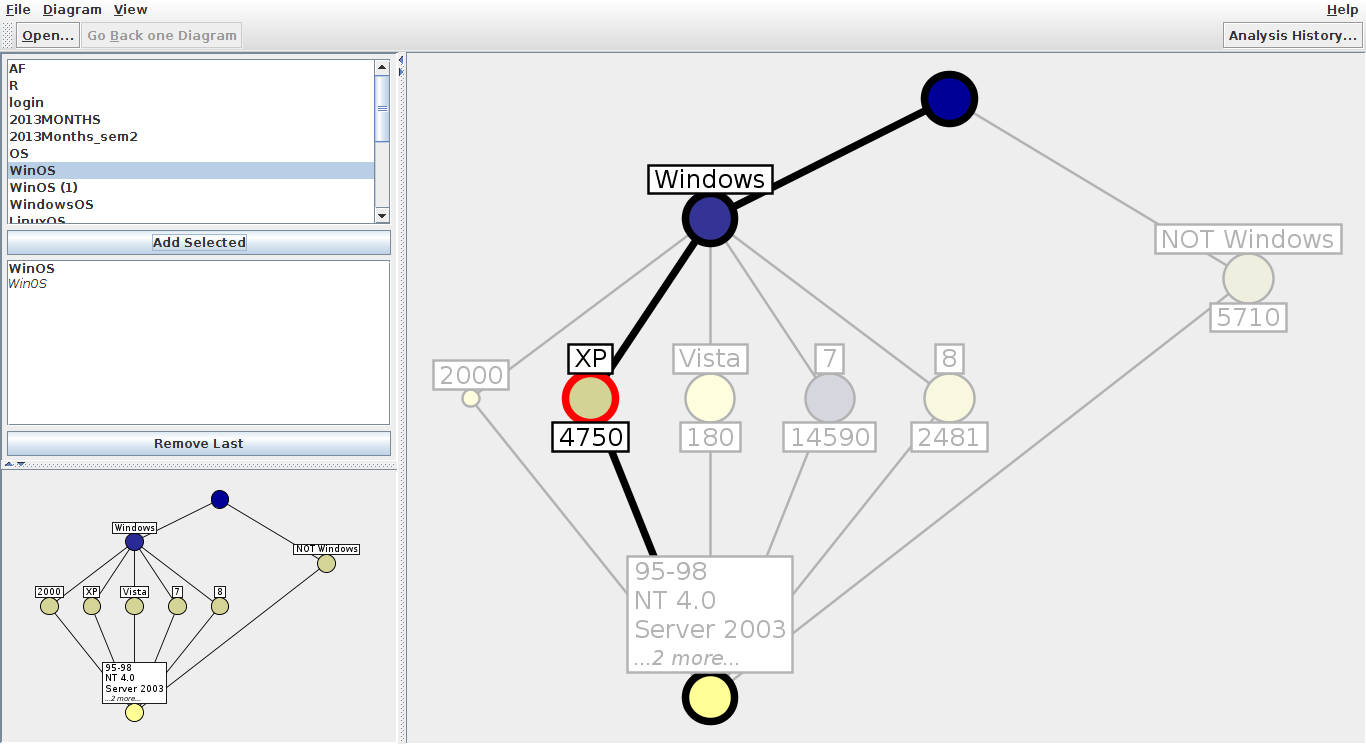
\includegraphics[width=\textwidth, natwidth=1366, natheight=744]{toscanaj-1.png} \\ 
          \caption{ToscanaJ, afișând o latice simplă generată din date de acces ale unui site web}
          \label{screenshot:toscana-1}
        \end{figure}
        \begin{figure}[h]
          \centering
          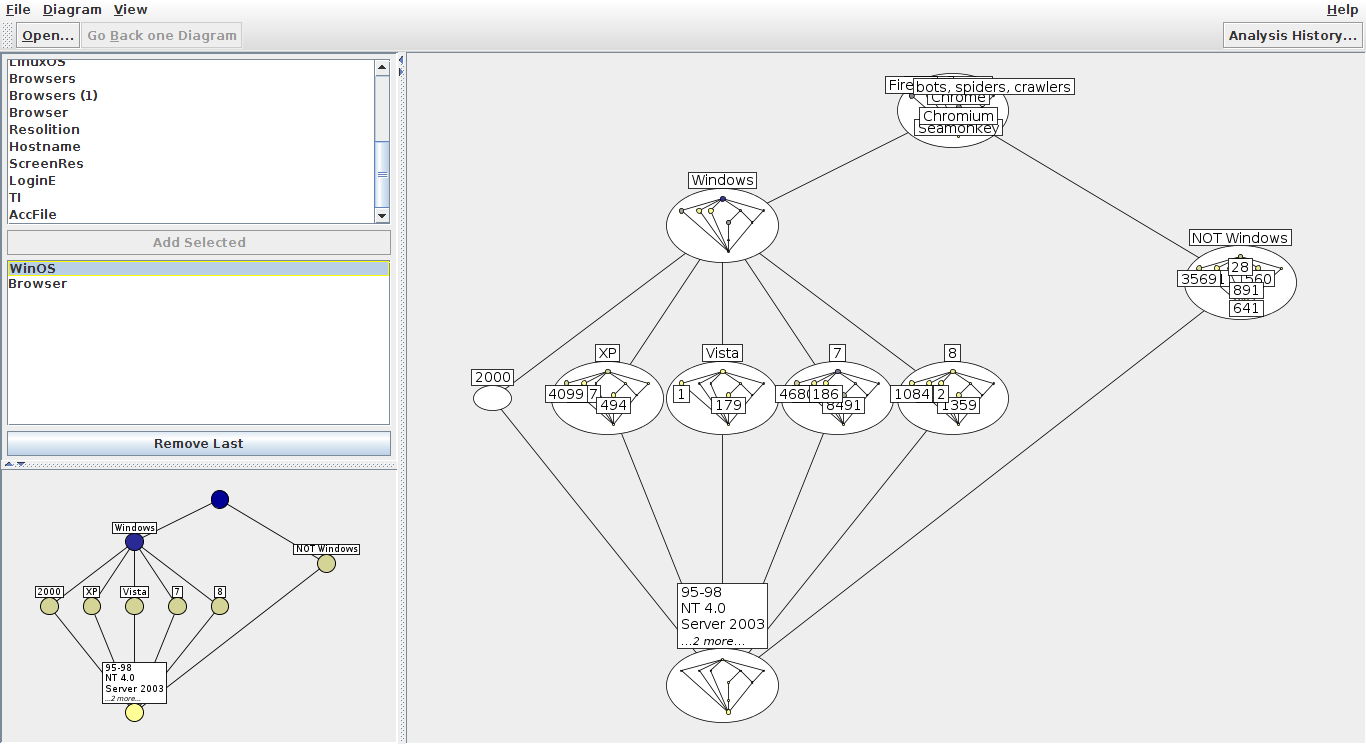
\includegraphics[width=\textwidth, natwidth=1366, natheight=744]{toscanaj-2.png}
          \caption{ToscanaJ, afișând aceeași latice ca în \ref{screenshot:toscana-1}, de data aceasta imbricată cu altă diagramă}
          \label{screenshot:toscana-2}
        \end{figure}

        Interfața ToscanaJ este punctul de pornire pentru Romagna. Vom încerca să păstrăm anumite elemente comune, pentru a ajuta utilizatorii obișnuiți, dar vom face, bine-nțeles schimbări și adaptări, mai ales luând în considerare diferențele convențiilor dintre interfețele aplicațiilor web, și cele desktop.

        ToscanaJ este, asemenea Romagna, doar un navigator de concepte. Modelarea conceptelor din date este realizată cu ajutorul altor programe din suita din care face parte și ToscanaJ.

        \begin{description}
            \item[Elba] este un editor pentru schemele conceptuale, legat de baze de date.
            \item[Siena] este un editor pentru scheme conceptuale, foarte asemănător cu \textbf{Elba}, diferența fiind că Siena nu are nevoie de o legătură cu o bază de date, putând descrie concepte simple direct în program.
        \end{description}

  \subsection{GaloisExplorer}
    GaloisExplorer \cite{GaloisExplorer:homepage} este un program mai recent, cu ultima actualizare în 2009.

    Are o interfață realizată în QT, ceea ce îi permite să funcționeze pe mai multe platforme. O abordare interesantă, dar în cele din urmă doar cu valoare estetică, este prezentarea laticelor în 3d (\ref{screenshot:galoisexplorer}).
   
    Din păcate, folosește anumite librării 3d (coin3d\cite{Coin:homepage}) care nu sunt imediat disponibile și care necesită compilare manuală.

    Pentru mulți utilizatori care nu au cunoștințe avansate de calculatoare, aceste impedimente sunt motiv suficient pentru a abandona această instalare.
    \begin{figure}[h]
      \centering
      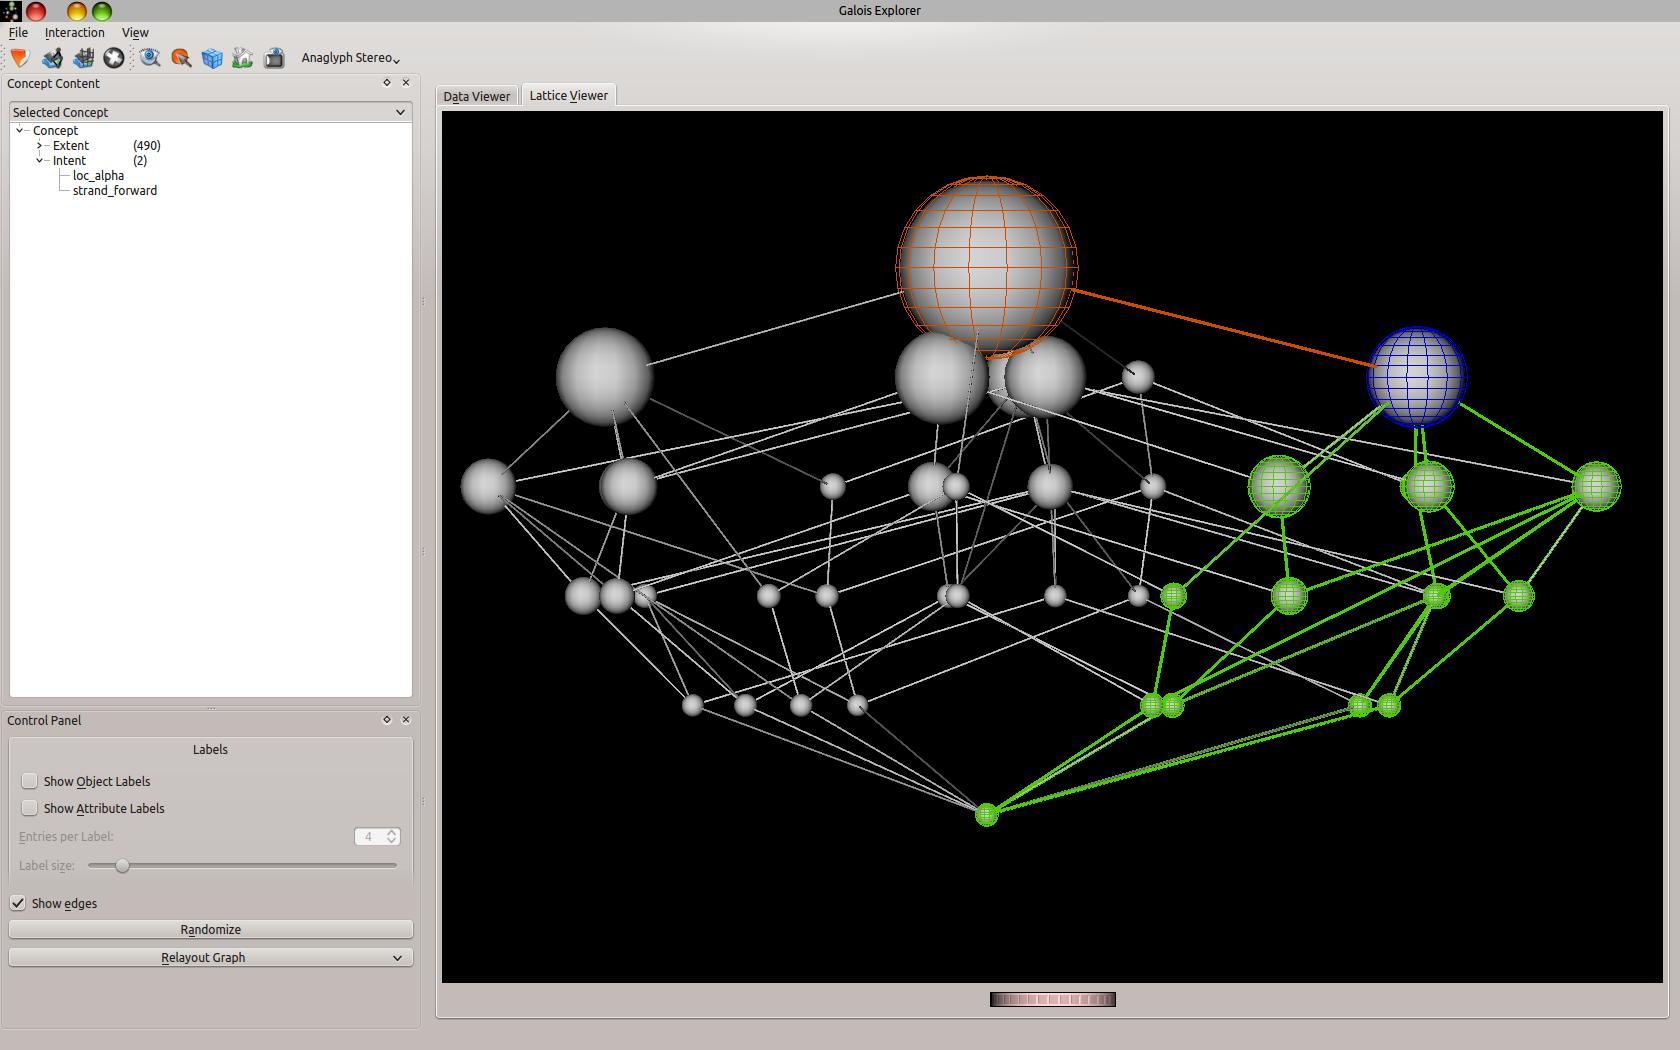
\includegraphics[width=\textwidth]{GaloisExplorer_latticeView}
      \caption{GaloisExplorer, afișând o diagramă în 3d. Sursa: site-ul proiectului \cite{GaloisExplorer:sourceforge}}
      \label{screenshot:galoisexplorer}
    \end{figure}

    \subsection{Galicia}
      Galicia este o aplicație Java dezvoltată la Universitatea din Montreal care dorește să acopere toate funcționalitățile necesare lucrului cu latice și contexte. Permite atât construcția și editarea contextelor, cât și vizualizarea 1aticilor rezultate.
  \section{Software conex}

    În această secțiune vom prezenta câteva alte programe remarcabile în domeniul FCA, sau care au avut un impact indirect asupra dezvoltării Romagna:
    \begin{description}
      \item[FCAStone] dezvoltat de Uta Priss, e un program care urmărește obținerea inter-operabilității între diferite programe pentru FCA (numele vine de la Piatra \textit{[n.t. Stone = Piatră]} Rosetta). Astfel, convertește fișierele folosite de mai multe suite în FCA. Pe lângă asta, convertește contexte în latice de concepte, și latice de concepte în formate grafice (atât vectoriale cât și raster).
      \item[Conexp] dezvoltat de Serhiy A. Yevtushenko, este o unealtă scrisă în Java, folosită în principal în scopuri educaționale (dar nu numai), are numeroase funcționalități de modelare a contextelor, dintre care amintim (preluate de site-ul programului \cite{conexp:users}):
        \begin{itemize}
            \item calculează numărul de concepte formale dintr-un context dat
            \item calculează laticea de concepte
            \item permite explorarea atributelor
            \item calculează regulile de asociații
        \end{itemize}
      \item[conexp-clj] O reimplementare scrisă de Daniel Borchmann în limbajul de programare Clojure a programului de mai sus. Programul pune accentul pe linia de comandă și programarea interactivă în domeniul FCA. Recent a adăugat un modul de interfață grafică, încă în stadiul experimental.
      \item[OpenFCA] Este o suită de trei aplicații, din care Conflexplore este o aplicație bazată pe Flex, folosită pentru explorarea conceptelor, atât tabelar cât și printr-o formă simplă de latice de concepte.  
        \item[Lattice Miner] Este o aplicație scrisă în Java, bazată pe 3 module, pentru concepte, contexte și reguli de asociere. Având structură modulară, permite integrarea de plug-inuri. Suportă interoperabilitatea cu Galitia și ConExp.
      \item[\LaTeX for FCA] \cite{LatexForFCA:homepage} Plugin pentru \LaTeX, scris de Bernhard Ganter, oferă câteva ``environment''-uri noi, folosite și în această lucrare, care permite aranjarea ușoară în pagina a contextelor și a laticilor derivate din acestea.
    \end{description}

\chapter{Tehnologii folosite}
\label{sec:tehnlogii}

  După cum am menționat, Romagna se bazează pe tehnologii web. Vom continua prin a descrie sumar principalele librării/framework-uri folosite și un raționament scurt pentru existența lor în proiect.

  \section{Extinderea trăsăturilor de limbaj - CoffeeScript}
    Unul din principalele motive pentru care browser-ul nu a fost mult timp acceptat ca o platformă matură pentru aplicații era absența altor limbaje de programare disponibile înafară de JavaScript.

    Această stare de fapt se schimbă încet din mai multe motive:
    \begin{itemize}
      \item JavaScript a evoluat și este considerat un limbaj de programare mai matur decât în perioada în care a fost scris ToscanaJ.
      \item Existența \textbf{emscripten}, descris pe scurt în subsecțiunea \ref{subsec:emscripten} și rezultatele obținute de acesta.
      \item Existența limbajelor care compilează \textit{în} JavaScript.
    \end{itemize}

    Unul din aceste limbaje este \textbf{CoffeeScript} \cite{ashkenas:2012:coffeescript}. CoffeeScript nu introduce decât două concepte (clase versus prototipuri și array comprehensions) noi față de JavaScript, dar simplifică dezvoltarea prin câteva îmbunătățiri:
    \begin{itemize}
      \item Evitarea variabilelor globale
      \item Câteva scurtături de sintaxă (\verb=->= pentru a declara o funcție, \verb~=>~ pentru a declara o funcție legată de contextul actual, etc.) 
      \item Clarificarea operatorilor de comparație (\verb~==~ în CoffeeScript devine automat \verb~===~ în JavaScript, scăpând automat de o întreagă clase de erori).
    \end{itemize}
        Alături de sintaxa mai prietenoasă (o opinie personală a autorului), prin elidarea acoladelor în favoarea indentării pentru definirea blocurilor, am ales CoffeeScript ca limbajul principal pentru Romagna.

  \section{Scalabilitate și arhitectură corectă în aplicații web - Ember.js}
    Ember.js este un framework scris în JavaScript, inspirat de Cocoa, și are ca scop ușurarea dezvoltării aplicațiilor web complexe, prin oferirea unui cadru MVC, cu o structură relativ rigidă. 
    
    Inițial aplicația nu era bazată pe niciun framework. Pe măsură ce complexitatea structurii a crescut, am realizat că recreăm, involuntar, un sistem MVC, mai mult ca sigur imperfect.
   
    Am hotărât să reorganizăm codul în urma unei deliberări, bazându-ne pe faptul că un framework folosit de mii de oameni, cu teste funcționale și modulare la zi poate oferi o fundație puternică, fără a ne cheltui timpul ``reinventând roata''. Din variantele disponibile de framework-uri pentru JavaScript, am ales Ember.js deoarece:
    \begin{itemize}
      \item Structura impusă se potrivește cu necesitățile proiectului.
      \item Posibilitatea schimbării ușoare a adaptorului a repozitoriului de date inclus în framework înseamnă că vom putea crea o variantă viitoare a Romagna care se includă comunicarea cu un server, funcționalitate care este plănuită pentru versiuni care vor urma.
      \item Funcționalitatea componentei \verb=Router=, care permite crearea de URL-uri, care pot fi salvate de utilizator, în funcție de navigarea sa prin aplicație, înseamnă că avem la îndemână o formă simplă de serializare și salvare a stării aplicației.
    \end{itemize}
  \section{Manipularea documentelor și vizualizare de date - d3.js}
    D3 (provenit din \textit{Data-Driven Documents} - Documente Bazate pe Date) este o librărie scrisă în JavaScript pentru manipularea DOM-ului relaționând cu date legate de elemente din document. Citând din abstractul lucrării \cite{bostock:2011:d3}:
    \begin{quote}
      ``Cu D3, designerii leagă în mod selectiv date de intrare de elemente arbitrare ale documentului, aplicând transformări dinamice pentru a genera, cât și a modifica conținut.''
    \end{quote}
    Devine clar din descrierea de mai sus că această librărie va ușura dezvoltarea aplicației, datorită posibilității de a lega \textit{conceptele} de reprezentarea acestora într-un mod care să permită modificarea acestei reprezentări în funcție de explorarea diagramelor de către utilizator, ceea ce, este, până la urmă scopul aplicației.
    \subsection{Grafică scalabilă - svg}

      D3 se bazează pe manipularea DOM-ului pentru a obține vizualizări dinamice de date. Deși HTML-ul poate fi stilizat, formele complexe și imaginile vectoriale sunt descrise în browser prin SVG \cite{Ferraiolo:01:SVG}, un standard de grafică vectorială bazată pe XML. Deși ajută la crearea unor aplicații de vizualizare complexe, SVG-ul vine cu problemele sale, care sunt descrise mai pe larg în sub-subsecțiunea \ref{subsubsec:svg-problems}.
  \section{SQL în browser - sql.js}
    După cum am descris în secțiunea \ref{subsec:confidentiality}, pilonii pe care am decis să construim Romagna (ușurința utilizării și păstrarea locală a datelor) pun în dificultate folosirea unei arhitecturi client-server, deoarece vrem un proces de instalare și folosire cât mai simplu (nici un proces de instalare nu e mai simplu decât deschiderea unei pagini web), iar utilizatorii nu-și vor trimite datele unei părți terțe, din temeri proprii sau pentru că nu au acest drept, lucrând cu date confidențiale.

    Astfel, compromisul este de a analiza SQL în browser, cu ajutorul sql.js \cite{sqljs:homepage}, care este defapt SQLite recompilat în JavaScript cu ajutorul emscripten.

    SQL.js poate rula într-un Web Worker, echivalentul unui thread izolat folosit de JavaScript în browser \cite{Hickson:12:WW}. Astfel, operațiile de interogare asupra bazei de date nu au un impact direct asupra răspunsului interfeței.

    \subsection{Compilarea codului C/C++ în JavaScript - emscripten}
    \label{subsec:emscripten}
      Din abstractul articolului \cite{Zakai:2011:ELC:2048147.2048224}
      \begin{quote}
        ``[\ldots] prezentăm Emscripten, un compilator din limbaj de asamblare LLVM (Low Level Virtual Machine) în Javascript. Acesta deschide două căi de a rula cod scris în alte limbaje decât Javascript pe web: 1. Compilarea codului direct în limbaj de asamblare LLVM și apoi compilarea acestuia în JavaScript folosindu-vă de Emscripten, sau 2. compilarea întregului run-time al unui limbaj interpretat în LLVM și apoi în JavaScript.''
      \end{quote}

    Impactul pe care acest compilator l-a avut este, cel puțin până acum, unul mai mult teoretic, majoritatea programelor fiind folosite cu rol demonstrativ. Aplicațiile compilate în JavaScript sunt, bine-nțeles, mai lente decât variantele lor compilate direct în limbaj de asamblare. Totuși pentru o anumită categorie de programe, între care se află și Romagna, acest schimb de viteză pentru funcționalitățile oferite de librăria sau aplicația compilată este binevenit. Structurile de date folosite de Romagna până în acest moment nu sunt atât de mari încât pierderea performanței să fie critică.


\chapter{Romagna}
\label{chapter:3}

  Romagna este o aplicație dezvoltată începând cu anul 2014, pornită la Universitatea Babeș-Bolyai ca o alternativă folosindu-se de tehnologiile web pentru un navigator de concepte modern.

  Numele (Romagna) este o referință directă suitei de programe care a inspirat această aplicație, Toscana. Romagna este o regiune istorică a Italiei aflată la nordul Toscanei. 

  Pe lângă funcționalitățile ale aplicației ToscanaJ descrise în sub-subsecțiunea \ref{subsubsec:toscanaj-functionalitati}, Romagna are câteva funcționalități noi plănuite, descrise în secțiunea \ref{sec:future}.

  Dezvoltarea acestei aplicații are câteva scopuri \textit{(diferite de funcționalități)} principale, prezentate în secțiunea următoare.

  \section{Raționament}
  \label{sec:rationament}

    \subsection{Ușurința utilizării}
    \label{subsec:usurinta-de-utilizare}
      Uneltele destinate FCA trebuie gândite ca programe pentru consumatori, utilizatori obișnuiți. Publicul țintă al acestor aplicații nu sunt neapărat programatori sau oameni cu experiență în folosirea avansată a calculatoarelor. Oamenii care beneficiază cel mai mult de asemenea aplicații sunt cercetători în domenii foarte diferite (după cum se vede în secțiunea de aplicații practice \ref{sec:utilizari-practice})

      Din acest punct de vedere, este părerea autorului că soft-ul existent în acest domeniu nu satisface necesitățile publicului său țintă. 

      Pentru clarificare, următoarele puncte trebuie îndeplinite pentru a considera o aplicație ușor de folosit:
      \begin{itemize}
      \item Aplicația trebuie să fie \textbf{ușor de instalat}. Programatorii de multe ori scapă din vedere acest aspect, dacă nu e vorba de un produs comercial, care are nevoie de cât mai mulți utilizatori.
        E inadmisibil să se ceară compilarea manuală a unei librării C++, sau instalarea unui server MySQL unui utilizator obișnuit pentru a utiliza un program. Romagna, fiind o aplicație web, sare peste acești pași. Singurii pași premergători folosirii aplicației sunt pregătirea datelor pentru consum de către aplicație și familiarizarea cu interfața aplicației.
      \item Aplicația trebuie să fie \textbf{disponibilă pe mai multe platforme}. Utilizatorii nu vor instala un alt sistem de operare pentru a testa o aplicație. 
        În schimb, majoritatea utilizatorilor au la dispoziție un navigator web modern, cum ar fi Mozilla Firefox, Google Chrome, etc. 
        Aceste medii de aplicații (pentru că navigatoarele web și mediul de execuție al limbajului JavaScript pus la dispoziție de acestea a devenit un mediu de aplicații) se actualizează automat, permițând utilizarea celor mai noi funcționalități unei majorități a utilizatorilor acestora.
        \item Aplicația trebuie să ofere \textbf{date de ieșire utile} utilizatorului. Ne referim aici bine-nțeles la rezultatele așteptate de utilizator, prezentate într-un mod clar, dar și la mesajele de erori, care trebuie să fie inteligibile, să ofere cursuri de acțiune care să rezolve problema întâmpinată, într-un limbaj non-tehnic, pe cât posibil.
          Erorile criptice, cum ar fi stack-trace-uri, sau excepții afișate pe ecran descurajează utilizatorul obișnuit.
        \item Aplicația trebuie să aibă \textbf{o interfață plăcută}. E părerea autorului că, deși utilizabile, interfețele generate de aplicații Java în general oferă o experiență neplăcută, nu se integrează în stilul sistemului de operare. Aplicațiile web sunt mult mai ușor de estetizat, mai ales cu ajutorul unor framework-uri CSS, dintre care amintim Twitter Bootsrap sau Zurb Foundation.
          \item Ca o ultimă alternativă pentru utilizator, aplicația trebuie să vină \textbf{însoțită de documentație}. Aceasta trebuie formulată într-un limbaj non-tehnic.
          \item Opțional, aplicația ar trebui să aibă \textbf{interfața localizată}. Nu toți utilizatorii de calculatoare sunt vorbitori de engleză. Folosirea pictogramelor pentru realizarea interfeței poate ajuta, dar inclusiv în acest caz, diferențele culturale, sau conceptele prea complexe pe care dezvoltatorii încearcă să le transmită, pot descuraja utilizarea aplicației mai mult decât să ajute.
      \end{itemize}

      Romagna îndeplinește unele din condițiile de mai sus(ușor de instalat, ușor de găsit) prin natura aplicațiilor web, iar celelalte condiții constituie obiectul efortului autorului.

    \subsection{Folosirea web-ului, păstrarea confidențialității datelor}
    \label{subsec:confidentiality}

      Este o stare de fapt că în domeniul analizei datelor, integritatea și confidențialitatea acestora este o grijă constantă.

      Mulți cercetători lucrează de asemenea cu date care sunt, legal vorbind, secrete. Se înțelege astfel, că majoritatea potențialilor utilizatori \textbf{nu} vor avea încredere să trimită datele unui serviciu extern.

      Din aceste considerente, o arhitectură server peste web (și oferirea Romagnei ca serviciu) a fost imediat desconsiderată. Dar, cum am menționat în subsecțiunea \ref{subsec:usurinta-de-utilizare}, ușurința de utilizare este o altă calitate pe care încercăm să o regăsim în Romagna. 
      
      S-a ajuns astfel la compromisul (temporar) de a realiza \textbf{totul} în browser. Asta înseamnă accesarea datelor SQL în browser, prin tehnologii descrise în capitolul \ref{sec:tehnologii}.

  \section{Date de intrare}

    Datele de intrare pentru Romagna sunt (cel puțin în acest moment, pe viitor vom accepta mai multe tipuri de date) fișiere \verb=.csx=, fișiere XML care au o structură aproximativă:

    \begin{figure}[h!]
    \inputminted[fontsize=\footnotesize]{xml}{context.csx}
    \caption{Exemplu de sintaxă a unui fișier de intrare.}
    \end{figure}

    După cum se vede, fișierul e secționat în diagrame, care conțin conceptele ca și colecții de referințe către atribute și obiecte și muchii între concepte. Pentru brevitate, am emis elementele \textit{<objectElementStyle>} și \textit{<attributeELementStyle}, care descriu cum ar trebui desenată eticheta fiecărui atribut/obiect în parte.

    Dacă fișierul csx nu conține datele contextului, are nevoie de o bază de date. Aceasta este referențiată prin

    \begin{minted}{xml}
    <databaseConnection>
      <embed url="file:///home/calea/catre/baza_de_date.sql" />
        <table name="Tabel_relevant" />
        <key name="COOKIE_ID" />
    </databaseConnection>
    \end{minted}

  și referințele către obiecte/atribute se fac prin interogări care vor fi executate pe tabelul refernțiat mai sus. \mint{xml}|<object>((IPID>8) AND (IPID<=9)) AND ((IPID>30) AND (IPID<=40))</object>|

  \section{Structură}

    Structura la nivel înalt este ghidată de folosirea librăriei Ember.js. Aceasta impune dezvoltarea aplicației pe principiile MVC. Pe lângă aceste principii, cerințele specifice domeniului au dus la câteva deviații mici. 
    
    În mod normal accesul la date ar trebui să se facă \textit{exclusiv} printr-un repozitoriu de date, dar datorită naturii fișierelor csx, care permit interogări sql integrate în structura lor (după cum am arătat mai sus), controlorul are nevoie de acces direct la o bază de date, fără a accesa repozitoriul pus la dispoziție de Ember.

    Întrucât există mai multe variante ale formatului \verb=.csx= (nu este standardizat), primul pas este uniformizarea și prelucrarea datelor de intrare în structurile de date interne ale aplicației (care coincid în mare parte cu conceptele descrise în \ref{chapter:1} - modele care descriu \textit{contexte, concepte, atribute, obiecte, latice}). Pe lângă acestea, diagramele în sine sunt modele, și au controlori aferenți.
    \begin{figure}[h!]
      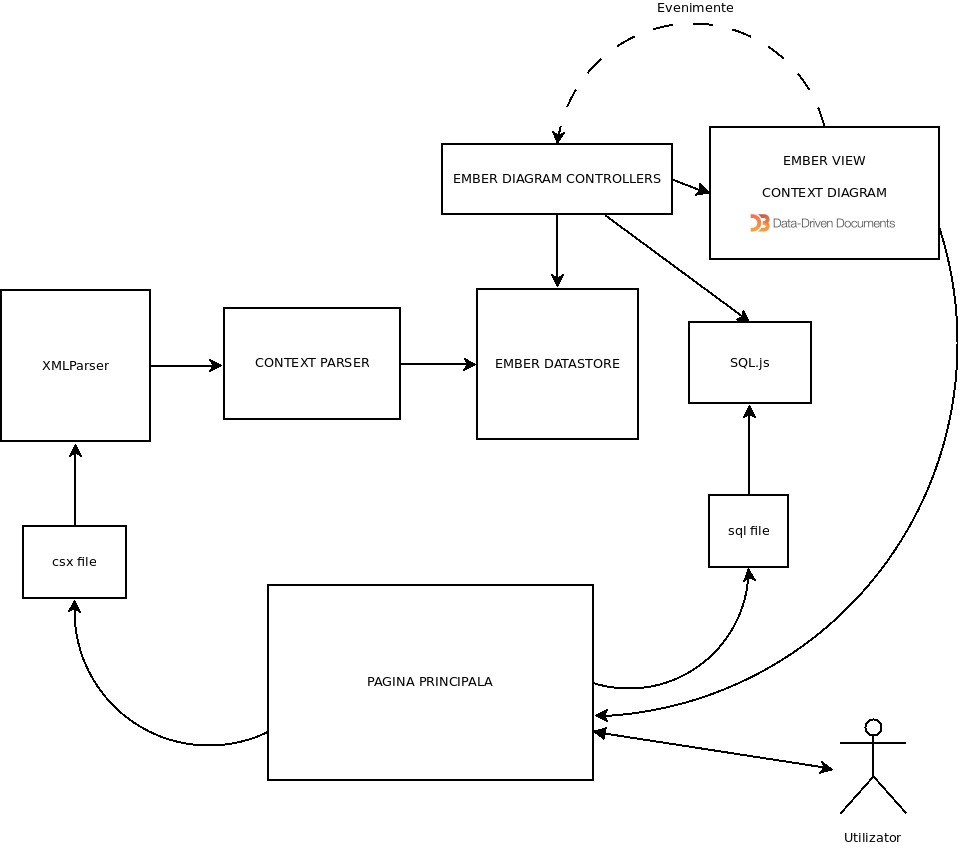
\includegraphics[width=\textwidth, natwidth=960, natheight=848]{romagna_architecture.png}
      \caption{Diagrama viziunii de ansamblu asupra arhitecturii aplicației Romagna}
    \end{figure}
    
    \textit{View}-ul, sau interfața diagramei este controlată de Ember doar în raport cu celelalte componente ale aplicației (mai specific cu controlorii, View-urile sunt, în MVC-ul clasic, pe care Ember îl respectă, limitate la a comunica cu controlorul); desenarea diagramei este făcută de către d3.js, iar tot el înregistrează evenimentele DOM, pe care le trimite mai departe la Ember, care, la rândul său, va interoga sql.js pentru date, sau își va interoga propriul repozitoriu de date, în cazul în care fișierul \verb=.csx= conținea toate datele contextului.
    
  \section{Dezvoltare}

    Dezvoltarea a început în anul 2014. Odată alese tehnologiile pe care am dezvoltat aplicația, primiii pași au fost studiere în detaliu a fișierelor \verb=.csx=, care sunt inputul principal al programului ToscanaJ.

    În figura \ref{screenshot:romagna:1} se vede o versiune incipientă a programului afișând o diagramă extrasă dintr-un fișier de exemplu al ToscanaJ.
    \begin{figure}[h]
      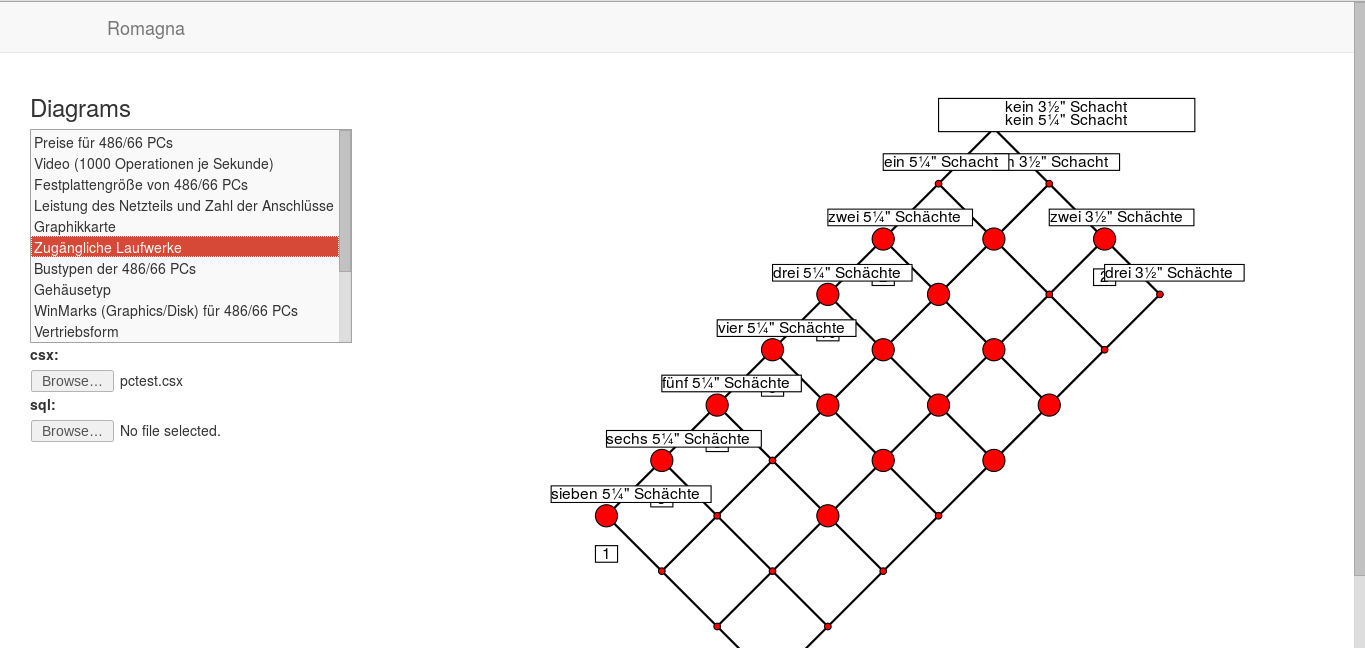
\includegraphics[width=\textwidth]{romagna-01.png}
      \caption{Versiunea 0.1 a aplicației, rulând pe Mozilla Firefox, versiunea 33, pe sistemul de operare Ubuntu Linux afișând o diagramă derivată dintr-un fișier de test inclus în arhiva descărcată cu ToscanaJ}
      \label{screenshot:romagna:1}
      \end{figure}
    \subsection{Probleme întâmpinate}
      
      \subsubsection{MySQL versus sql.js} % (fold)
      \label{ssub:MySQL versus sql.js}

        ToscanaJ folosește baza de date MySQL pentru interpretarea volumelor mai mari de date decât ar fi gestionabile în fișiere excel sau csv, etc. În schimb, Romagna folosește o variantă a SQLite.

      Din fericire, site-ul dezvoltatorilor SQLite oferă o listă \cite{sqlite:converters} de programe folosite pentru convertirea fișierelor de export MySQL în fișiere de folosit pentru SQLite.

      % subsubsection MySQL versus sql.js (end)
      \subsubsection{SVG și probleme în afișarea corectă a textului}
      \label{subsubsec:svg-problems}
        HTML-ul (mai ales folosit în tandem cu CSS), la fel ca și \LaTeX, de altfel, permite formatarea foarte ușoară a textului. Această proprietate derivă din scopul existenței sale ca un limbaj de formatare a documentelor interconectate.

        SVG-ul în schimb are ca scop descrierea imaginilor vectoriale. Astfel, textul nu are un rol special în acest standard; toate uneltele cu care browser-ul este dotat pentru încadrarea textului în containere nu sunt disponibile atunci când lucrăm cu svg, cum este în cazul nostru la afișarea diagramelor.

        Chiar dacă un element \verb=<text>= se află într-un container cum ar fi un element \verb=<rect>= sau \verb=<g>= și containerul are dimensiuni bine definite, textul se va revărsa înafara containerului, ceea ce va duce la un aspect foarte urât și la probleme grave de lizibilitate, după cum se poate observa din figura \ref{screenshot:svg-overflow}

        \begin{figure}[h]
            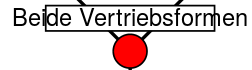
\includegraphics[width=.5\textwidth, natwidth=252, natheight=70]{svg-overflow.png}
            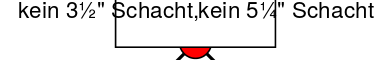
\includegraphics[width=.5\textwidth, natwidth=387, natheight=60]{svg-overflow-2.png}
            \caption{Captură de ecran din varianta 0.1 a aplicației, demonstrând text care se revarsă din containerul său.}
            \label{screenshot:svg-overflow}
          \end{figure}

        Rezolvarea acestor probleme implică calcularea constantă a lungimii textului, redimensionarea containerului, sau în cazul în care containerele sunt aglomerate micșorarea textului.

        De asemenea, începerea unui rând nou într-un element \verb=<text>= nu este posibilă printr-o secvență de caractere (cum este \verb=\n= în stringurile obișnuite, sau \verb=\\= în \LaTeX). Orice linie nouă trebuie introdusă într-un element nou \verb=<tspan>=, și poziționat manual.

        Astfel, multă muncă trebuie depusă în formatarea textului, un aspect care în celelalte părți ale dezvoltării web este rezolvat complet de platformă.


  \chapter*{Concluzii}
    Dezvoltarea aplicației nu este un proces încheiat (și este părerea autorului că în majoritatea cazurilor procesul de dezvoltare al software-ului nu se sfârșește niciodată), dar putem ajunge la niște concluzii. 

    \begin{enumerate}
        \item Analiza conceptuală formală este un câmp vast, din a cărui teorie am dezvoltat foarte puțin în această lucrare. Pentru mai multe detalii, recomandăm sursele citate în capitolul \ref{chapter:1} și ale cărei aplicații concrete sunt prea numeroase pentru a fi numerotate.
          \item Platforma web s-a dovedit a fi una potrivită pentru provocarea pe care o reprezintă navigarea conceptelor unui context.
          \item Deși aplicația funcționează, în sensul de a avea \textit{funcționalitățile} propuse, una din provocările pe care ni le-am propus când am început acest proiect a fost să creăm o aplicație care să fie plăcută de cercetători și de amatori de vizualizare. Întrucât proiectul nu a fost făcut public până acum, nu putem confirma că am reușit în această privință.
    \end{enumerate}

  \section*{Viitor}
  \label{sec:future}
    Dezvoltarea Romagna va continua în trei direcții mari în viitor:
    \begin{description}
        \item [Rafinarea interfeței existente] Pentru primele versiuni a aplicației am pus accent pe o interfață cât mai simplă, de-a dreptul spartană. Vom continua prin a aduce îmbunătățiri cum ar fi funcționalitate pentru taburi, pentru a permite utilizatorilor explorarea mai multor subcontexte al aceluiași context simultan.

          Alte îmbunătățiri planificate țin de posibilitatea explorării unei latice prin zoom și prin metode de focalizare+context, descrise în subsecțiunea \ref{subsubsec:focalizare}.

        \item [Dezvoltarea unui editor live de contexte, cu răspuns imediat în afișarea diagramei] O unealtă care, în opinia autorului, ar fi \textit{foarte} utilă în scopuri didactice și exploratorii. A putea vedea direct implicațiile pe care schimbarea valorii unui atribut asupra unui obiect le are asupra contextului și laticei poate ajuta înțelegerea domeniului foarte mult de către studenți și amatori. Putem extinde acest concept după aceea la folosirea aplicației pentru dezvoltarea unei pagini complexe de prezentare a analizei conceptuale formale studenților, cu cursuri interactive direct în browser.

          Această funcționalitate necesită însă un efort de dezvoltare foarte mare, deoarece pentru a prezenta aceste schimbări în timp real, fără a duce la frustrarea utilizatorului necesită algoritmi foarte eficienți de conversie a contextului în latice și de a reprezenta laticea (și schimbările acesteia).


        \item [Editarea contextului \textit{din} diagramă] În mod obișnuit diagrama are doar rol de prezentare. Dar putem să ne gândim la un caz de utilizare unde editarea contextului este posibilă direct din latice.

        \item[Dezvoltarea unui convertor automat din MySQL în SQLite] - Momentan conversia datelor este un proces separat, pe care-l cerem utilizatorilor de ToscanaJ care doresc să încerce aplicația noastră. Acest pas în plus poate fi destul pentru anumiți utilizatori să renunțe să încerce aplicația noastră.

        \item [Dezvoltarea unei componente server] Actuala configurație a întregii activități desfășurate în browser este un compromis, apărut în urma cerințelor. Un server dedicat găzduirii și procesării bazei de date va permite folosirea programului pentru seturi de date prea mari pentru a fi încărcate în browser. 

          Dezvoltarea în această direcție este dependentă de răspunsul din partea utilizatorilor.
    \end{description}

    Deși dezvoltarea a început ca un proiect de diplomă, autorul pune codul sursă la dispoziția oricui și încurajează colaborarea și/sau dezvoltarea în paralel pentru diferite necesități. Repozitoriul canonic se află pe site-ul de găzduire a software-ului Github \cite{Romagna:repo}, unde veți găsi informații curente despre dezvoltarea Romagnei.

\bibliographystyle{alpha}
\bibliography{romagna}
\appendix
\end{document}
